\chapter {Cloud Approach}
In this chapter of the proposal we introduce the collective entity matching problem and give our solution to implement it on the cloud. We start by giving a motivating example, theoretical foundation, and then we explain the different components of our solution.

\section{Simple Example}
As an example we use a bibliographical example presented by Bhattacharya and Getoor\cite{BhGe06b}. In this example we consider the problem of resolving the authors in academic publications databases like DBLP and CiteSeer. Consider the following set of four papers:

\begin{enumerate}
\item A. V. Aho, S. C. Johnson, J. D. Ullman, "code generation for machines with multi-register operations"
\item A. V. Aho, J. D. Ullman, "The university of database languages"
\item A. V. Aho, J. D. Ullman, "Optical partial-match retrieval when fields are independently specified"
\item Alfredo V. Aho, Jeffrey D. Ullman, Scott Johnson, "Code generation for expressions with common sub-expressions"
\end{enumerate}

We would like to find out, given these papers, which of the referenced author names belong to the same author entities. For instance we need to determine whether paper 1 and paper 2 are written by the same author named Ullman, or whether the name references belong to different authors. The same need to be considered for the Ullman from paper 3 and Ullman from paper 4, and all pairwise combinations. Similar questions about the author names Johnson and Aho also need to be considered in this context. 

In order to resolve these authors references, we may begin by examining the author references to see which ones we consider to be the same. In the first step we might decide that all of the Aho references refer to the same author entity because Aho is an unusual last name. This corresponds to resolving all the Aho references into a single entity. However, we might be not quite sure that the Ullman references are the same author, and we certainly not sure about Johnson references, since Johnson is very common name. But deciding that the Aho references correspond to the same entity gives us additional information for the Ullman references. We know that the references share a common co-author. Now with the higher confidence we can consolidate the Ullman references. Based solely on the Aho entity consolidation, we do not have enough evidence to consolidate the Johnson references. However, after making the Ullman consolidations, we may decide that having two co-authors in common is enough evidence to tip the balance, and that all the Johnson references correspond to the same Johnson entity Figure \ref{fig:shaded_ref}.b.

In this example, it turns out there are three author entities. We will call these entities \textit{Alfred V Aho} and \textit{Jeffrey D Ullman}, and \textit{Scott Johnson}. This is illustrated by figure ~\ref{fig:shaded_ref}(b), where references correspond to the same authors are shaded identically.

\begin{figure}
\centering
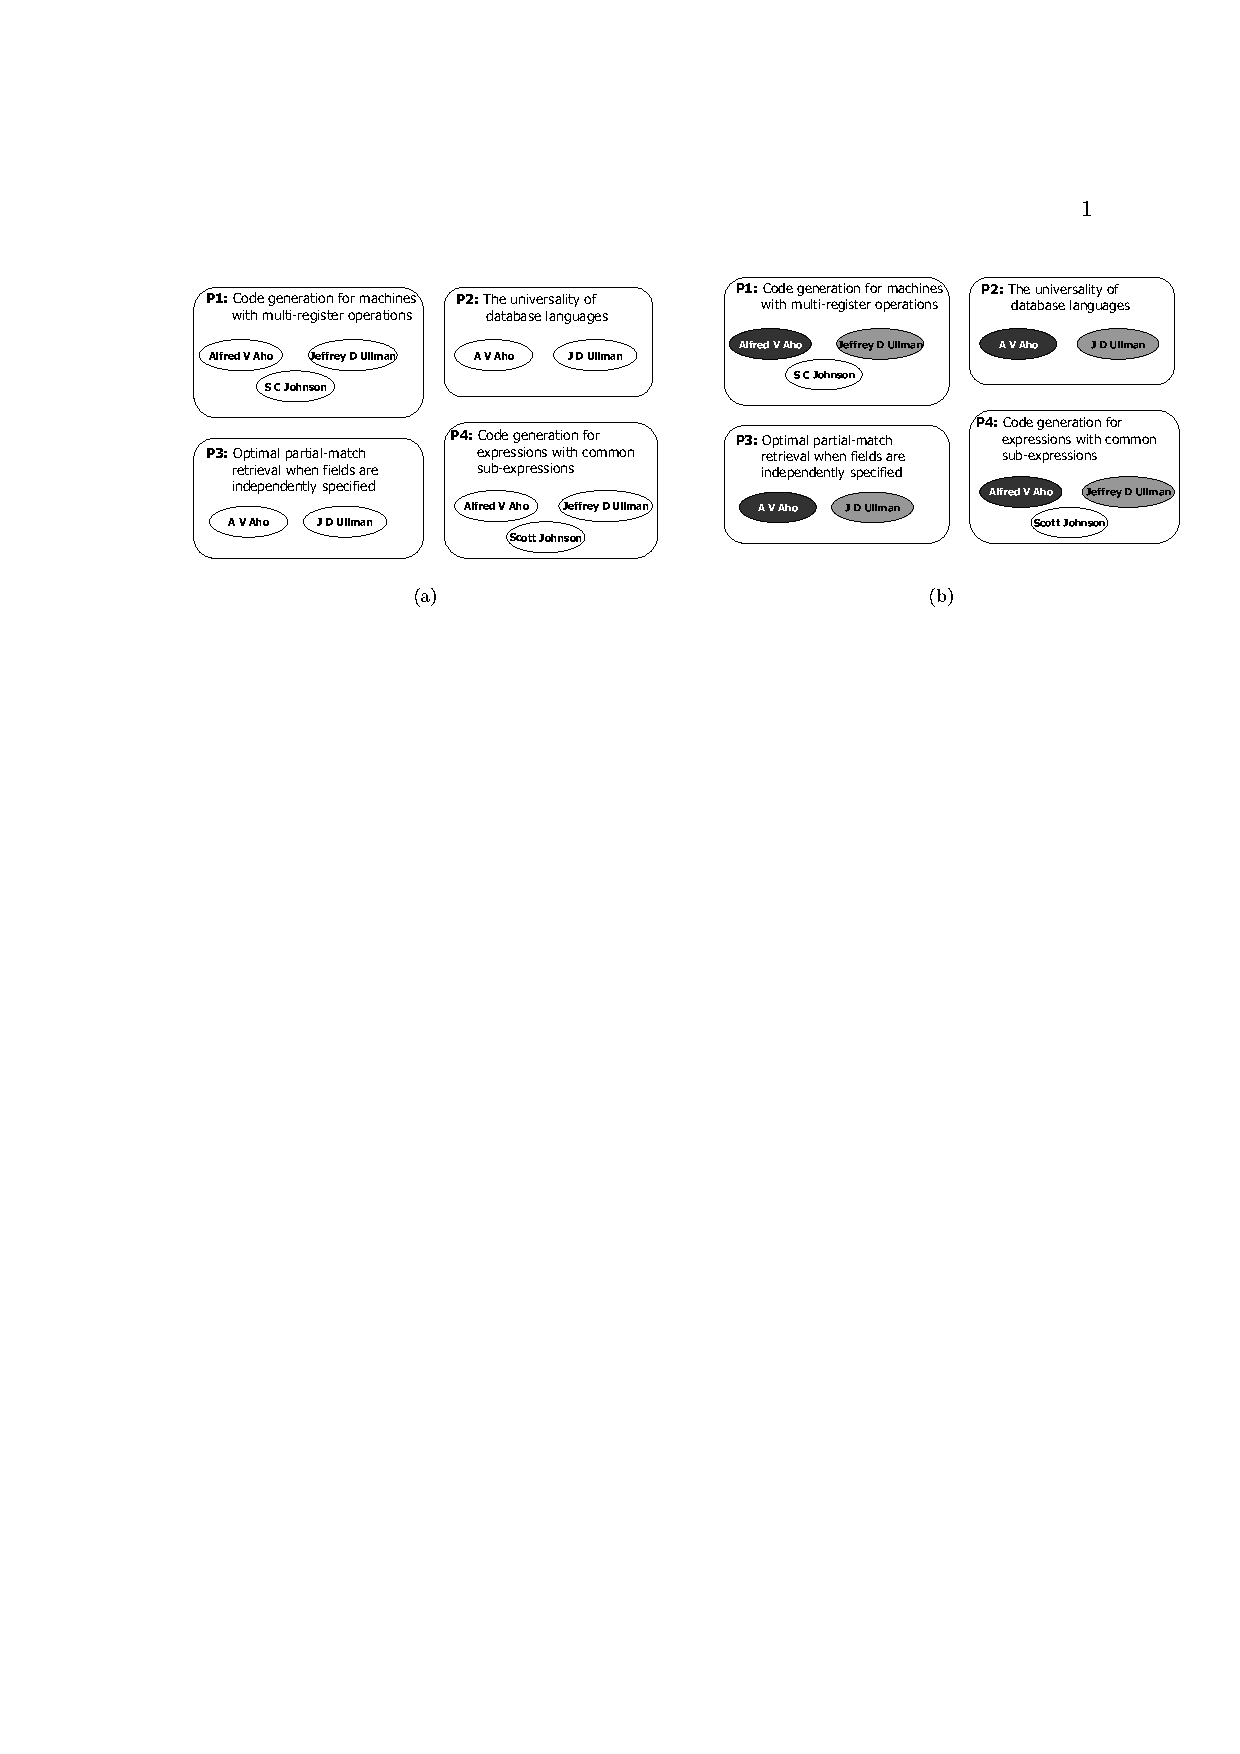
\includegraphics[page=1,trim = 32mm 190mm 0mm 45mm, clip]{figures/chapter3/fig1_ab_cliping}  
\caption{(a) An example author/paper resolution problem. Each box represents a paper reference and each oval represents an author reference. (b) The resolved entities corresponding to the example author/paper resolution problem. (\cite{BhGe06b})}
\label{fig:shaded_ref}
\end{figure}  

In this example we can find instances of the identification problem. The identification problem can be seen in the references with different names which refer to the same entity. For example entity author 'Jeffery David Ullman' might be referenced as 'J. D. Ullman', 'Jeffery D. Ullman', 'J. Ullman' and so on.

To solve identification and disambiguation problems, relationships between references can be used to better resolve the references to their corresponding real entities \cite{BhGe07}. These relationships can be represented as a graph where nodes represent the references and the hyper-edges represent the relationships between references. In our example the graph can be constructed by letting the nodes represent the authors and the hyper-edges represent the co-authorship relation that hold between them. Figure ~\ref{fig:ref_ent}(a) shows the reference graph for our bibliographic example.

Given this graph representation for our data, our goal is to take into consideration the hyper-edges to better partition the references into entities. This is because references with similar or exact names are more likely to be the same entity if their hyper-edges connect to the same entities as well. We can see this in our example (figure ~\ref{fig:shaded_ref}), first observe that the Ullman references collaborate with Aho's who correspond to the same author. This makes it more likely that they are the same entity. From the relationship graph between the references we incrementally constructs the entity graph by considering as evidence the entity relationships that it has already discovered earlier. Figure ~\ref{fig:ref_ent}(b) shows the resulting entity graph for our example after all the references have been correctly resolved.

\begin{figure}%[ht!]
\centering
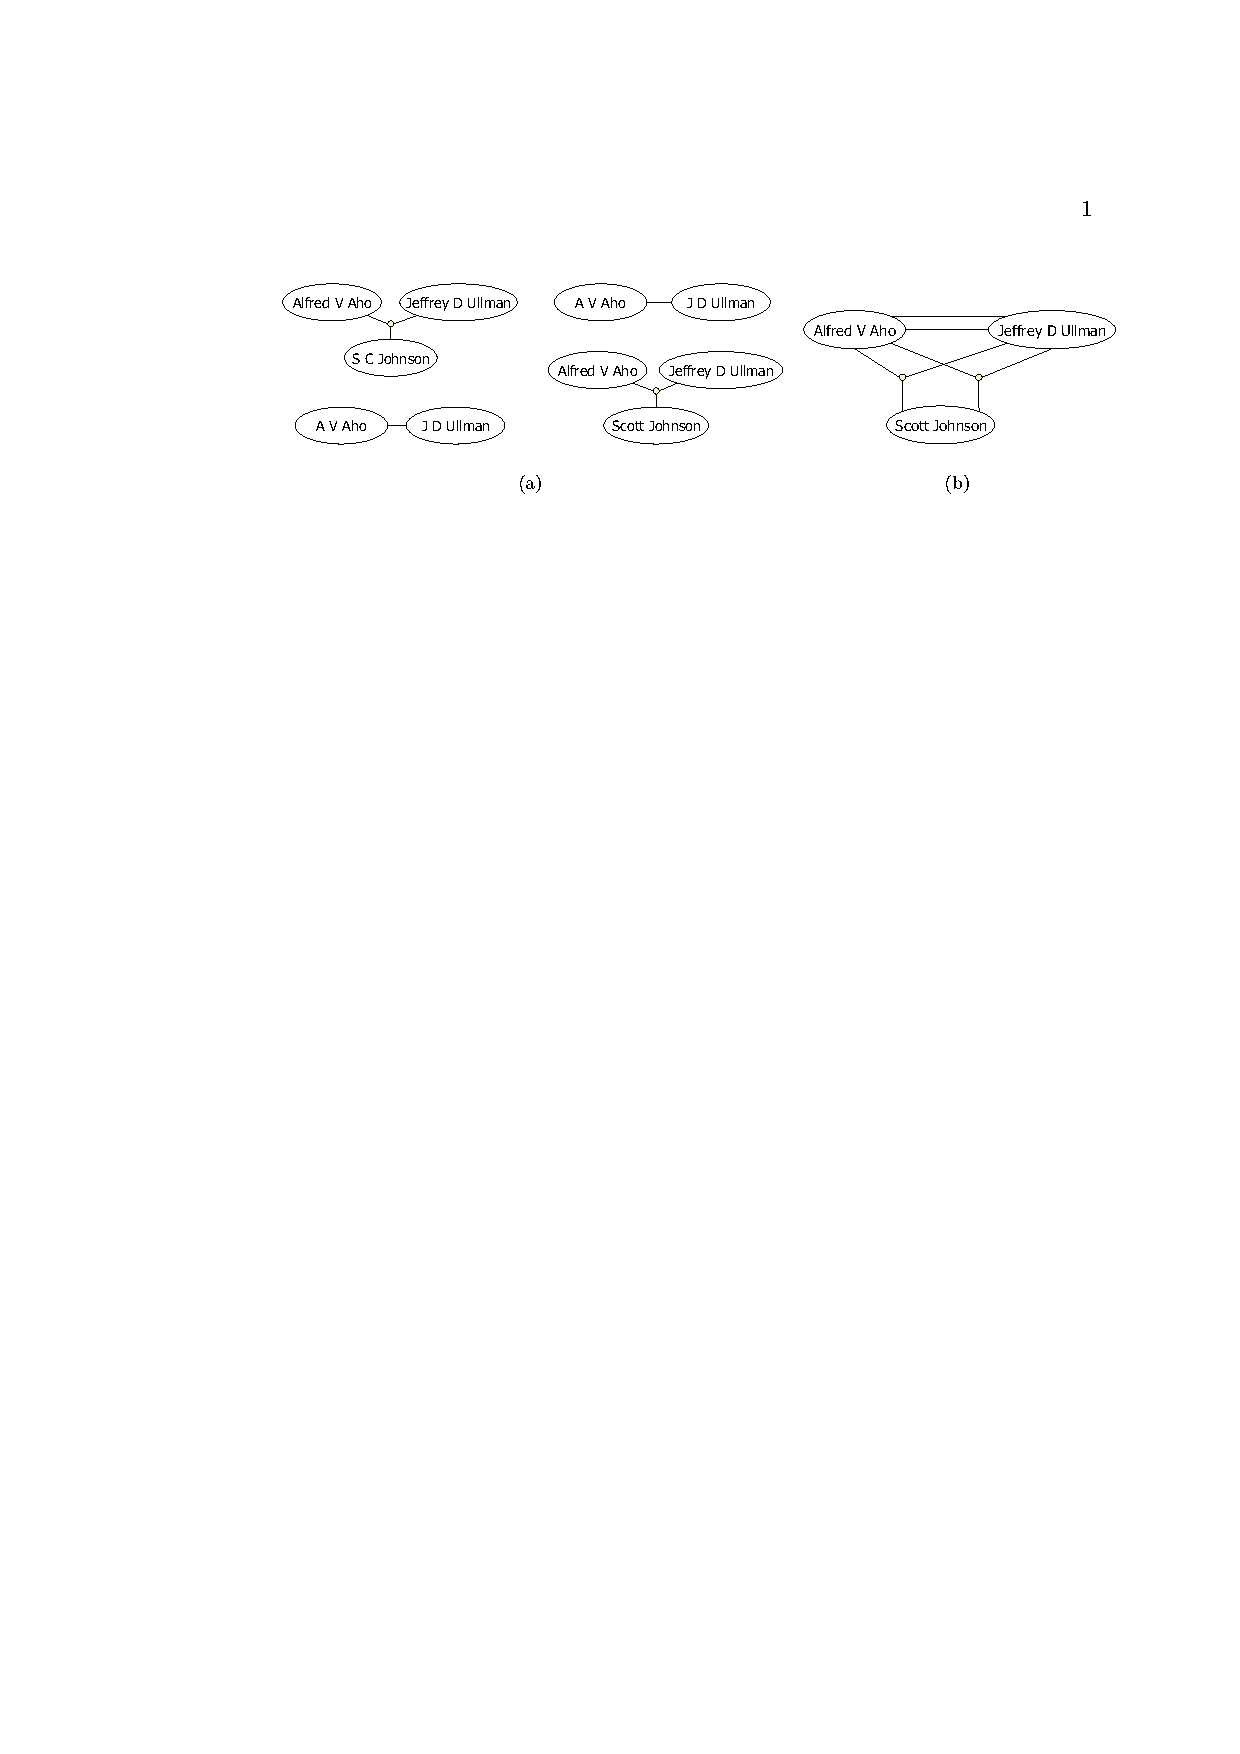
\includegraphics[page=1,trim = 35mm 210mm 0mm 45mm, clip]{figures/chapter3/fig2_ab_cliping}
\caption{(a) The reference graph and (b) the entity graph for the author resolution example. (\cite{BhGe07})}
\label{fig:ref_ent}
\end{figure}  

\section{Theoretical Foundation}

In this section, we introduce the notation to be used for describing the relational entity resolution problem based on the work of Bhattacharya and Getoor\cite{BhGe07}.
 
To formalize the problem we need notations for references, entities and hyper-edges. In the entity resolution problem, we are given a set of references $\mathcal{R}=\{r_i\}$, where each reference $r$ has attributes $r.A_1,r.A_2,...,r.A_k$. The references correspond to some set of unknown entities $\mathcal{E} = \{e_i\}$. We introduce the notation $r.E$ to refer to the entity to which reference $r$ corresponds.

 The problem is to recover the hidden set of entities $\mathcal{E} = \{e_i\}$ and the entity labels $r.E$ for individual references given the observed attributes of the references.In the context of collective entity matching, we assume that the references are not observed independently, but that they co-occur. We describe the co-occurrence with a set of hyper-edges $\mathcal{H} =\{h_i\}$. Each hyper-edge h may have attributes as well, which we denote $h.A_1,h.A_2,...,h.A_l$, and we use $h.R$ to denote the set of references that it connects. A reference $r$ can belong to zero or more hyper-edges and we use $r.H$ to denote the set of hyper-edges in which $r$ participates. Considering again out example, we can see how this notation is represented.

Lets show how this applies to our example, Figure \ref{fig:abs_ent}(a) shows the references and hyper-edges. Since each author name corresponds to a reference, then there are ten references $r_1$ through $r_{10}$. In this case, the the attributes are the names themselves, so for example $r_1.A$ is "Alfred Aho", $r_2.A$ is "S. C. Johnson" and $r_3.A$ is "Jeffrey Ullman". Now considering the entities, we have a set of true entities as shown in figure \ref{fig:abs_ent}(b). where $e_1.A=$"Alfred V. Aho", $e_2.A=$"S. C. Johnson" and $e_3.A=$"Jeffrey D. Ullman". We observe that references $r_1$, $r_4$, $r_6$ and $r_8$ correspond to "Alfred V. Aho", so that $r_1.E = r_4.E = r_6.E = r_8.E = e_1$. In similar way, we observe that $r.3:E = r_5.E = r_7.E = r_10 = e_2$ and $r_2.E = r_9.E = e_3$. 
Now considering the Hyper-edges, we have hyper-edges $\mathcal{H} = \{h_1,h_2,h_3,h_4\}$, one for each paper. The attributes of  the hyper-edges in this domain are the paper titles; for example, $h_1.A_1=$"Code generation for machines with multi-register operations". The references $r_1$ through $r_3$ are associated with hyper-edge $h_1$, since they are the observed author references in the first paper. This is represented as $h_1.R = \{r_1,r_2,r_3\}$. We similarly represent the hyper-edge associations of the other references. The problem here is to figure out from the attributes $r.A$ and the hyper-edge label $r.h$ of the references that there are three distinct entities such that $r_1,r_4,4_6$ and $r_8$ corresponds to one entity, $r_3,r_5,r_7$ and $r_10$ correspond to the second entity and $r_2$ and $r_9$ correspond to the third. Here we have introduced the notation assuming that all references correspond to the same class of entities, It may be extended to handle multiple entity classes and multiple types of hyper-edges between references.

\begin{figure}%[ht!]
\centering
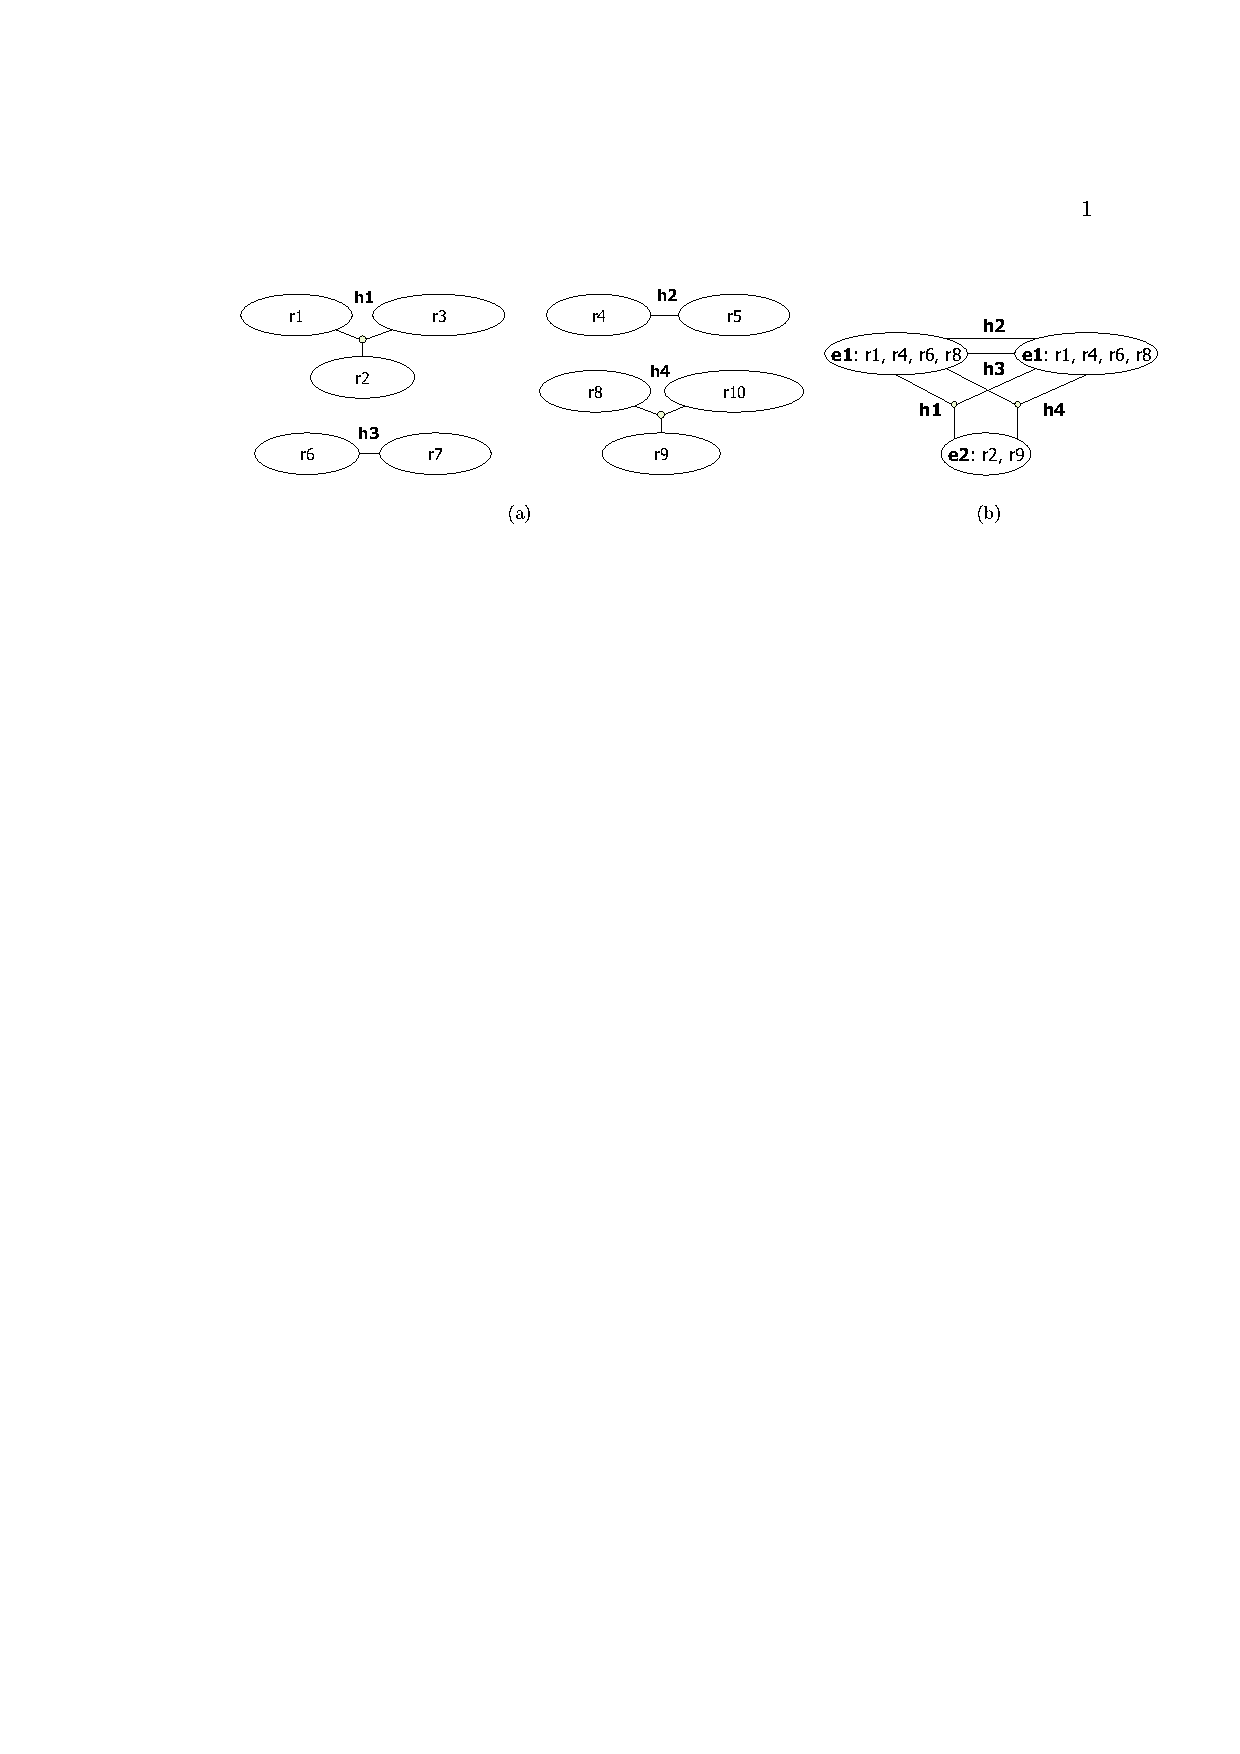
\includegraphics[page=1,trim = 35mm 205mm 0mm 45mm, clip]{figures/chapter3/fig3_ab_cliping} 
\caption{(a) A more abstract representation of the reference graph for the author resolution example; the r's are references and the h's are hyper-edges. (b) An abstract representation for the entity graph for the author resolution example; the nodes are the entities, the set of references they correspond to are listed, and the h's are hyper-edges.. (\cite{BhGe07})}
\label{fig:abs_ent}
\end{figure}  
\section{Proposed Solution}
In this section we describe the solution approach . The solution approach consists of several stages as shown in figure \ref{fig:SolutionAppraoch}. We give an overview of each stage and discuss the problems need to be solved in each stage.

\begin{figure} [H]
\centering
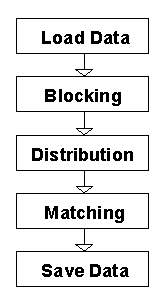
\includegraphics{figures/chapter3/fig0_ApproachBlockDiagram.eps}  
\caption{Block Diagram of the Solution Approach}
\label{fig:SolutionAppraoch}
\end{figure}

\subsection{Load Data}
In load data stage. Data from different sources having different formats need to be loaded into the framework.
\subsection{Blocking}
In this stage, the loaded data need to be blocked such that similar entities are grouped into blocks. The blocks may overlap with each other. Figure \ref{fig:bloking_example} shows the references to authors grouped into blocks.

\begin{figure}[H]
\centering
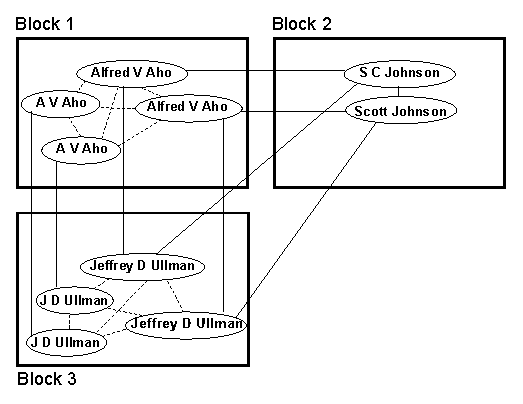
\includegraphics{figures/chapter3/fig_blocking_example.eps}  
\caption{Blocking of the reference graph (solid: links to neighbor references, dashed: links to references in the same block) }
\label{fig:bloking_example}
\end{figure}

\subsection{Distribution}
After the data records are grouped to overlapped blocks (canopies), we need to distribute the data over the machines of the cloud. the distribution should be balanced and should also ensure that overlapped blocks reside in the same machine. To illustrate that we added more author references to our running example. The new author references are grouped in \textit{block4} and \textit{block5}. \textit{block5} overlaps with both \textit{block2} and \textit{block4}. The blocks are distributed among two machines such that overlapped blocks resides in single machine and the blocks distribution among the two machines is balanced as much as possible (see figure \ref{fig:distributedBlocks_example}).

\begin{figure}[H]
\centering
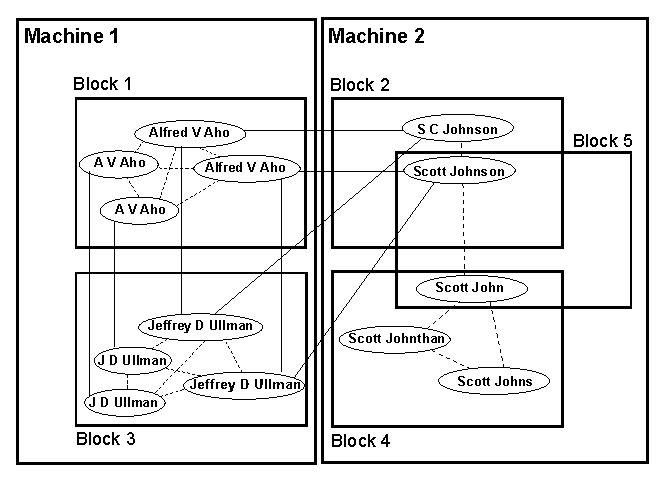
\includegraphics{figures/chapter3/fig_overlapedBlocks_machines.eps}  
\caption{Overlapped blocks should reside in single machine}
\label{fig:distributedBlocks_example}
\end{figure}


\subsection{Matching}
In this stage, the blocked data records that have similarity measure above the user defined threshold will be merged. We use the Collective relational entity matching approach and implement it on Pregel.
\subsection{Save Data}
After the data is matched, we need to store the results. statistical and log files should also be stored.

\section{Blocking By Canopies on MapReduce}
%all algorithms from \cite{SPYa10}
We use canopies for blocking stage. Canopies\cite{MNUn00} are overlapping subsets of high-dimensional dataset that is divided efficiently by using a cheap, approximate distance measures. An element may appear under more than one canopy, and every element must appear in at least one canopy. Canopies are created with the intention that points not appearing in any common canopy are far enough apart that they could not possibly be in the same cluster. Since the distance measure used to create canopies is approximate, there may not be a guarantee of this property, but by allowing canopies to overlap with each other, by choosing a large enough distance threshold, and by understanding the properties of the approximate distance measure, we can have a guarantee in some cases. 

When creating the canopies, given a distance metric, we should make sure that no two canopies are created with too much overlaps. The creation of canopies is as follows. we start with a list of the data points in any order, and with two distance thresholds, T1 and T2, where T1 $>$ T2. (These thresholds can be set by the user, or selected by cross-validation), we pick a point off the list and approximately measure its distance to all other points. We put all points that are within distance threshold T1 into a canopy. Then we remove from the list all points that are within distance threshold T2. We repeat until the list is empty\cite{MNUn00}. Figure \ref{alg:createCanopies_singleMachine} gives the algorithm for canopies creation.

\begin{figure}[H]
% \SetAlgoLined
1 \hspace{5ex}Input: points, threshold T1, T2 where T1$>$T2\\
2 \hspace{5ex}Output: cluster centroids\\
3 \hspace{5ex}Put all points into a queue Q\\
4 \hspace{5ex}While (Q is not empty)\\
5 \hspace{10ex}p = dequeue(Q)\\
6 \hspace{10ex}For each canopy c:\\
7 \hspace{15ex}if dist(p,c)$<$ T1: c.add(p)\\
8 \hspace{15ex}if dist(p,c)$<$ T2: strongBound= true\\
9 \hspace{10ex}If not strongBound: create canopy at p\\
10 \hspace{4ex}For all canopy c:\\
11 \hspace{9ex}Set centroid to the mean of all points in c\\
\caption{Canopy creation algorithm \cite{SPYa10}}
\label{alg:createCanopies_singleMachine}
\end{figure} 

We can implement the create canopies on MapReduce. 
\begin{figure}[H]
% \SetAlgoLined
\hspace{3ex} \textbf{Map()}\\
1 \hspace{5ex}Input: A set of points P, threshold T1, T2\\
2 \hspace{5ex}Output: key = null; value = a list of local canopies (total, count)\\
3 \hspace{5ex}For each p in P:\\
4 \hspace{10ex}For each canopy c:\\
5 \hspace{15ex}if dist(p,c)$<$ T1 then c.total+=p, c.count++\\
6 \hspace{15ex}if dist(p,c)$<$ T2 then strongBound= true\\
7 \hspace{15ex}If not strongBound then create canopy at p\\ 
8 \hspace{3ex}\textbf{Close()}\\
8 \hspace{5ex}For each canopy c:\\
9 \hspace{10ex}Emit(null, (total, count))\\
\caption{steps inside the Map  of the create canopy}
\label{fig:map}
\end{figure} 

\begin{figure}[H]
% \SetAlgoLined
\hspace{3ex} \textbf{Reduce()}\\
1 \hspace{5ex}Input: key = null; input values (total, count)\\
2 \hspace{5ex}Output: key = null; value = cluster centroids\\
3 \hspace{5ex}For each intermediate values\\
4 \hspace{10ex}p = total/count\\
5 \hspace{10ex}For each canopy c:\\
6 \hspace{15ex}if dist(p,c)$<$ T1 then c.total+=p, c.count++;\\
7 \hspace{15ex}if dist(p,c)$<$ T2 then strongBound= true\\ 
8 \hspace{10ex}If not strongBound then create canopy at p\\
9 \hspace{5ex} \textbf{Close()}\\
10 \hspace{9ex}For each canopy c: emit(null, c.total/c.count)\\
\caption{steps inside the Reduce of the create canopy}
\label{fig:reduce}
\end{figure} 

\begin{figure}[H]
% \SetAlgoLined
\hspace{3ex} \textbf{Map()}\\
1 \hspace{5ex}Input: Point p; cluster centriods\\
2 \hspace{5ex}Output: Output key = cluster id, Output value =point id\\
3 \hspace{5ex}currentDist= inf\\
4 \hspace{5ex}For each cluster centroids c\\
5 \hspace{10ex}If dist(p,c)<currentDist then bestCluster=c, currentDist=dist(p,c);\\
6 \hspace{5ex}Emit(bestCluster, p)\\
\caption{steps inside the Map of the cluster assignment}
\label{fig:map}
\end{figure} 

\section{Distribution}
\begin{comment}
Assume that we have 2 machines and 5 block $b_1,b_2,...,b_5$. $b_1$ overlaps with $b_2$ and $b_3$. The blocks elements are as follows:\\ 
$b_1=\{a,b,c,d\}$\\
$b_2=\{a,b,e\}$\\ 
$b_3=\{c,f,g\}$\\
$b_4=\{o,p,q,r,s\}$\\  
$b_5=\{w,y,z\}$\\

Since the blocks $b_1$,$b_2$ and $b_3$ overlaps, they should reside in one machine. The other blocks that do not overlap with each other can reside in any other machine. since we aim to have balanced distribution, they reside in the second machine. figure \ref{fig:fig_distribution_example} shows the required distribution of the blocks.
\begin{figure}[H]
\centering
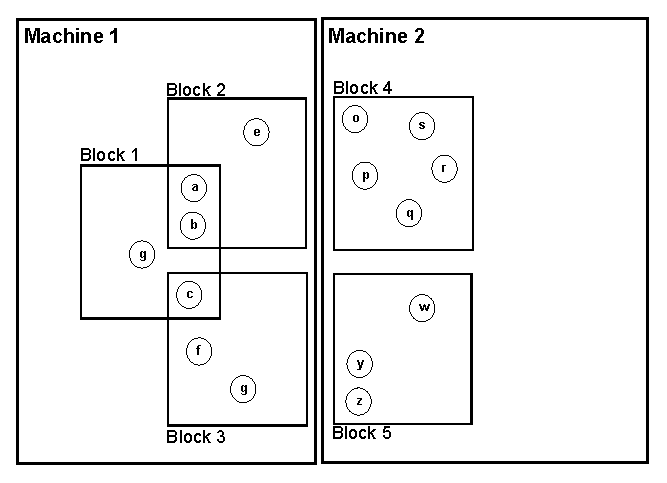
\includegraphics{figures/chapter3/fig_distribution_example.eps}  
\caption{overlapped blocks should reside in single machine}
\label{fig:fig_distribution_example}
\end{figure}
\end{comment}
Good partitioning of input data is a key prerequisite for parallel entity matching since it influences processor utilization, communication overhead, and load balancing\cite{KKH*10}. Since our algorithm is communication intensive, having good data partitioning is critical to have a local communication overhead centered in the machines of the cloud such that networking overhead is minimized.

To partition the input data we use a block-based partitioning approach proposed by Kirsten et. al. \cite{KKH*10}. This approach is called \textit{partition tuning} and it split or combine blocks as following:
\begin{itemize}
\item We start by determining all large blocks for which the memory requirements exceed the maximum allowed size. We split these block into several equally sized partitions that obey the size restriction.
\item Then we aggregate all smaller blocks that have size below some fraction of the maximal partition size into larger ones.
\end{itemize}



\section{Matching by Collective Relational Entity Matching}
Our solution approach is based on the collective relational entity matching introduced by Bhattacharya and Getoor\cite{BhGe07}. The main key idea of collective relational entity resolution,  is that resolutions are not made independently, but instead one resolution decision affects other resolutions via hyper-edges\cite{BhGe06b}.
 
In this approach, a relationship graph is built where references are represented as nodes and relationships between these references are represented as edges between corresponding nodes. The edges can be between more than two nodes (called hyper-edges). The similarity between two nodes is calculated as the weighted sum between attribute value similarity and the relational similarity. The relational similarity is calculated based on the connectivity of the two nodes through their hyper-edges as well as the connectivity of the neighboring nodes they are connected to. For collective entity resolution, we define the similarity of two clusters $c_i$ and $c_j$ as\cite{BhGe06b}:

%\begin{align*}
$$sim(c_i,c_j)=(1-\alpha) \times sim_A(c_i,c_j) + \alpha \times sim_R(c_i,c_j), 0\leq\alpha\leq1$$
%\end{align*}

where $sim_A()$ is the similarity of attributes and $sim_R()$ is the relational similarity between references in the two entity clusters. The relational similarity $sim_R()$ is dynamic in nature, which is one of the most important and interesting aspects of the collective approach\cite{BhGe07}. Worth to notice here that for collective resolution, the similarity of two clusters depends on the current cluster labels of their neighbors, and therefore changes as their labels are updated.

For collective entity resolution, relational similarity considers the cluster labels of all these connected references. Recall that each reference $r$ is associated with one or more hyper-edges in $\mathcal{H}$. Therefore, the set of hyper-edges $c.H$ that we need to consider for an entity cluster c is defined as\cite{BhGe07}:
%\begin{align*}
$$c.H= \bigcup_{r\in R \wedge r.C=c}\{h|h\in \mathcal{H} \wedge r \in h.R\}$$
%\end{align*} 
Cluster $c$ is connected to other clusters by these hyper-edges. For any cluster $c$, the set of other clusters to which $c$ is connected via its hyper-edge set $c.H$ form the neighborhood $Nbr(c)$ of cluster $c$\cite{BhGe07}:
%\begin{align*}
$$Nbr(c)= \bigcup_{h\in c.H,r\in h.R}\{c_j|c_j=r.C\}$$
%\end{align*} 

\begin{comment}
%This defines the neighborhood as a set of related clusters.
\subsection{Attribute Similarity Measures}
As we see, we need to measure the similarity of the attributes. A wide variety of measures exists. They can be categorized to character-based similarity measures, token-based similarity measures, phonetic similarity measures and numeric similarity measures \cite{EIV07}. We use SimMetrics, which is a Similarity Metric Library, that provide several measures from edit distance's (Levenshtein, Gotoh, Jaro etc) to other metrics, (e.g Soundex, Chapman). 
Specific Attribute similarity measures that is important to us are the following:

\subsubsection{Soft TF-IDF}
Soft TF-IDF similarity can be used for names since it has been shown to perform well for name-based entity resolution. Essentially, Soft TF-IDF augments the TF-IDF similarity for matching token sets with approximate token matching using a secondary string similarity measure \cite{BhGe07}.

\subsubsection{Jaro-Winkler}
Jaro-Winkler is reported to be the best secondary similarity measure for Soft TF-IDF. It is well-suited for short strings such as personal names \cite{BhGe07}

\subsubsection{Scaled Levenstein}
Scaled Levenstein belongs to the edit-distance family of similarity measures that assigns unit cost to each edit operation and normalizes the result \cite{BhGe07}.

\subsubsection{Cosine similarity}

\subsection{Neighborhood Similarity Measures} 
As we have seen, the relational similarity between two clusters can be calculated by the considering the similarity of their neighborhoods. Many different metrics have been proposed and evaluated in literature. In this section introduce some these measures and study their applicability for entity matching\cite{BhGe07}. 
\subsubsection{Common Neighbors}
This metric is the simplest approach. It measures the commomness between sets as well as counts the number of elements that occur in both. For two clusters $c_i$ and $c_j$, their common neighbor score is defined as\cite{BhGe07}
%\begin{align*}
$$CommonNbrScore(c_i,c_j)=\frac{1}{K} \times |Nbr(c_i)\bigcap Nbr(c_j)|$$
%\end{align*}
where $K$ is large enough constant such that the measure is less than 1 for all pairs of clusters. This measure is useful when the attribute similarity is not very informative since it measures the overlap in the reference's connected entities. The greater the number of common entities, the higher the possibility that the two references refer to the same entity as well. Note that this definition ignores the frequency of connectivity to a neighbor. We can define the measure to take into account the frequencies of occurrences of common clusters in the neighborhoods\cite{BhGe07}:
%\begin{align*}
$$CommonNbrScore+Fr(c_i,c_j)=\frac{1}{K'} \times |Nbr_B(c_i)\bigcap Nbr_B(c_j)|$$
%\end{align*}
The main shortcoming of this measure score is the normalizing constant $K$ that keep the same constant value over all pairs of clusters.

\subsubsection{Jaccard Coefficient}
This measure take into account the size of the neighborhood. This becomes important when entities are having large neighborhoods which leads to more likely finding shared neighbor by chance. this meausre is defined for two clusters as\cite{BhGe07}:
%\begin{align*}
$$JaccardCoeff(c_i,c_j)=\frac{|Nbr(c_i)\cap Nbr(c_j)|}{|Nbr(c_i)\cup Nbr(c_j)|}$$
%\end{align*}
Note that this definition ignores the frequency of connectivity to a neighbor. We can define the measure to take into account the frequencies of occurrences of common clusters in the neighborhoods\cite{BhGe07}:
%\begin{align*}
$$JaccardCoeff+Fr(c_i,c_j)=\frac{|Nbr_B(c_i)\cap Nbr_B(c_j)|}{|Nbr_B(c_i)\cup Nbr_C(c_j)|}$$
%\end{align*}
\subsubsection{Adamic/Adar Similarity}
The two measures we explained above consider all cluster labels in the neighborhood as equally important and significant for determining co-reference. However, when the cluster is frequently linked with many different clusters, then its presence in a shared neighborhood is not as significant as a cluster which is less frequent. We can introduce the 'uniquness' of cluster label $c$ and denote is as $u(c)$, then Adamic similarity score of two clusters $c_i$ and $c_j$ is defined as\cite{BhGe07}:

$$Adar(c_i,c_j)=\frac{\sum_{c\in Nbr(c_i)\cap Nbr(c_j)} u(c)}{\sum_{c\in Nbr(c_i)\cup Nbr(c_j)}}$$

\subsubsection{Adar Similarity with Ambiguity Estimate}

\subsubsection{Higher-Order Neighborhoods}
\end{comment}

\section{Vertex-oriented Collective Relational Clustering Algorithm}
As we already seen, Bhattacharya and Lise \cite{BhGe07} introduced an algorithm for relational clustering (see Figure \ref{fig:RC}). They used greedy agglomerative algorithm that finds the closest cluster pair at each step and merge them. On the other hand, Rastogi et. al. \cite{RDGa11} proposed a principled framework to scale any generic entity matching algorithm by running a collective matching process many times on small subsets of records that are in the same neighborhood of the data. These independent collective matching instances exchange messages about the local matches found, and the results of all matching instances are combined into a final overall solution\cite{Chri12}. They reported an implementation of the framework on MapReduce.

We combine the collective relational entity matching approach with the ideas of scalable distributed entity matching with message passing to develop a cloud-based framework and implement it using Pregel programming model. Figure \ref{fig:VRC} gives high level description of our algorithm that is written to be vertex-oriented.

\begin{figure}[H]
 \SetAlgoLined
1 \hspace{4ex} Find similar references using blocking\\
2 \hspace{5ex}Initialize clusters using bootstrapping\\
3 \hspace{5ex}For clusters $c_i,c_j$ such that similar($c_i,c_j$)\\
4 \hspace{10ex}Insert $<sim(c_i,c_j),c_i,c_j>$ into priority queue\\
5 \hspace{5ex}While priority queue not empty\\
6 \hspace{10ex}Extract $<sim(ci,cj),c_i,c_j>$ from queue\\
7 \hspace{10ex}If $<sim(c_i,c_j)>$ less than threshold, then stop\\
8 \hspace{10ex}Merge $c_i$ and $c_j$ to new cluster $c_{ij}$\\
9 \hspace{10ex}Remove entries for $c_i$ and $c_j$ from queue\\
10 \hspace{9ex}For each cluster $c_k$ such that similar($c_{ij},c_k)$\\
11 \hspace{20ex}Insert $<sim(c_{ij},c_k),c_{ij},c_k>$ into queue\\
12 \hspace{9ex}For each cluster $c_n$ neighbor of $c_{ij}$\\
13 \hspace{20ex}For $c_k$ such that similar($c_k,c_n$)\\
14 \hspace{28ex}Update $sim(c_k,c_n)$ in queue\\
\caption{High-level description of the relational clustering algorithm by Bhattacharya and Lise \cite{BhGe07}}
\label{fig:RC}
\end{figure} 

\begin{figure} [H]
 \SetAlgoLined
1 \hspace{5ex} Find similar references using blocking\\
2 \hspace{5ex} Build the reference graph\\
3 \hspace{5ex} For each block of references\\ 
4 \hspace{10ex}		Add an edge between each two nodes in the block\\ 
5 \hspace{5ex} Initialize clustering, each cluster contains single reference\\
6 \hspace{5ex} For each block do\\
7 \hspace{10ex}		Find the two clusters with the highest similarity\\
8 \hspace{10ex}		If the highest similarity is above user threshold\\ 
9 \hspace{15ex}			Merge the clusters that have highest similarity\\
10 \hspace{14ex}		Notify all neighbor clusters of the new merged cluster\\
11 \hspace{9ex}		Else\\ 
12 \hspace{14ex}		Exit\\
13 \hspace{9ex}		End If\\
14 \hspace{4ex} For each cluster that is notified from step 10\\
15 \hspace{9ex}		Re-calculate similarity between references of the cluster block\\ 
16 \hspace{5ex}Go to step 6\\ 
\caption{High-level description of the vertex-oriented relational clustering algorithm}
\label{fig:VRC}
\end{figure} 
 
In our algorithm, we implement the relational clustering algorithm of collective entity matching introduced by Bhattacharya and Lise \cite{BhGe07}. However, since this algorithm is not suitable for a cloud computing platform like Pregel, we need to re-write the relational clustering algorithm considering Pregel's vertex-oriented model of computing. In Pregel, programs are expressed as a sequence of iterations. In each iteration, a vertex can, independently of other vertices, receive messages sent to it in the previous iteration, send messages to other vertices, modify its own and its outgoing edges states, and mutate the graph's topology. In other words, we need to think like a vertex. 

Next we explain the algorithm steps in more details. For the implementation on cloud, we use MapReduce for step 1, and Pregel like system for the rest of steps.

In step 1, references are assigned to buckets using an attribute similarity measure. Each bucket has a representative reference that is the most similar to all references currently in the bucket. A naive implementation algorithm yields a $O(n(b+f))$ for $n$ references and $b$ buckets and when a reference is assigned to at most $f$ buckets. This can be improved by maintaining an inverted index over buckets. For example, when dealing with names, for each character we maintain the list of buckets storing last names starting with that character. Then the buckets can be looked up in constant time for each reference leading to an $O(nf)$ algorithm\cite{BhGe07}.

In step 2, references graph is built (see Figure \ref{fig:VRCillustrate}). In this graph, the references nodes are connected by two types of edges. The first type is relation edges (the solid line in the figure). The second type of the edges connects every two nodes within each block (the dashed lines in the figure). We need to add the block edges because nodes within each block need to exchange messages during the entity matching process, in Pregel, message exchange between nodes is possible only through edges. 
\begin{figure}
\centering
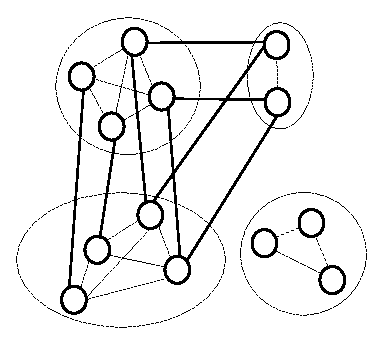
\includegraphics{figures/chapter3/fig_VRCillustrate.eps}  
\caption{References graph (solid-lines: relation edge , dashed-line: block edge)}
\label{fig:VRCillustrate}
\end{figure}

In step 3, the clustering is initialized by simply putting each reference node in single node cluster such that every reference has its own cluster. This is different from the original relational clustering algorithm where relational bootstrapping is necessary. In the initialization step, two lists are initialized in each node. The first list, we call the neighborhood list, contains information of the relational neighbor clusters. The second list,we call block list, contains information of the clusters that are in the same block that the node is.   

In step 4, the hierarchical agglomerative clustering start in each block. In each block, the two clusters having the highest similarity between them are searched. The search is restricted within each block. If the highest similarity is above the user-specified threshold, the two clusters are merged. upon merging the two clusters, all the relational neighbors (connected by relational edges) are notified. when implementing the hierarchical agglomerative clustering in Pregel model, we need to follow the following steps:
\begin{itemize}
\item Finding the two clusters that have the highest similarity measure requires that each node communicates to all the other nodes within the same block. The method follows the following supersteps:
\begin{itemize}
\item In the first superstep, each node sends its attribute information as well as the information of its relational neighbor clusters to all other nodes in the block (by querying the block list). These information is used by the target node to compute the attribute and the relational similarity such that each node compute the similarity between it self and every other node in the block.
\item In the second superstep, each node propagate the highest similarity measure value computed by itself. When the other nodes receives this similarity measure value, they compare it to the values of similarity measure computed by them selves. If the receiving node finds that highest similarity value that is received from all the nodes, if this value exists within its computation then the node recognize that it has the highest similarity between it self and another cluster within the block, otherwise the node does nothing.
\item In the third superstep, the two clusters with the highest similarity between them merges into new cluster. This requires unifying the cluster label, In addition, some extra work need to be done: 
\begin{itemize}
\item The neighborhood list of the new cluster need to be constructed by concatenating the neighborhood lists of the two merged clusters.

\item The block list of the new cluster need to be constructed by copying the block list from one of the merged clusters

\item The other clusters in the block need to update their block list by removing the entries of the old merged clusters and adding the entry of the new cluster

\item The relational neighbor clusters need to update their neighbor lists by removing the entries of the old merged clusters and adding the entry of the new cluster

\item Since the merge of clusters changes the relational structure of the reference graph, this effects the relational similarity, therefore the computation within all the blocks that include one of the relational neighbor clusters of the new cluster need to be done again. In fact this step gives the collective feature for the entity matching process. 
\end{itemize} 
\end{itemize}
\end{itemize}

Data partitioning is very important issue for the efficiency of our algorithm. We should aim for reducing the network overhead by having the blocks, each located completely in the same machine. Ideally, By assuring that data block are not distributed in many machines, we can have processing locally centered in each machine with minimum network traffic that is needed only when merging clusters since their neighbor clusters that need to be notified reside in other machines.
 